% There should be a better way to program vector graphics in LaTeX

\begin{figure}
\centering

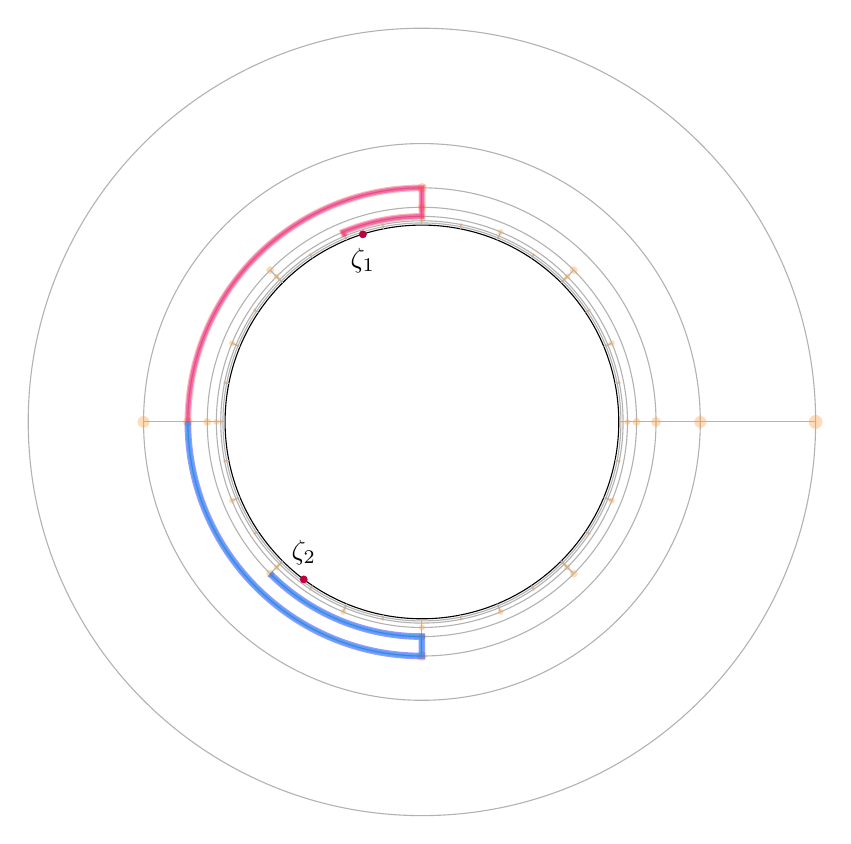
\begin{tikzpicture}[scale=2.5]
		
% The circles C_n
\draw (0,0) circle (1);
\foreach \i in {1,(1.0/2),(1.0/4),(1.0/8), (1.0/16), (1.0/32), (1.0/64)}{
\draw[black!30!white] (0,0) circle (2^\i);
}
   
\foreach \j in {0,1,2,3,4,5}{
    \pgfmathsetmacro{\jtwo}{2.0^\j}
    \pgfmathsetmacro{\jthree}{(1.0/\jtwo)}
    \pgfmathsetmacro{\twopower}{2^\jthree}
    \foreach \angleone in {1,...,\jtwo}{
    \pgfmathsetmacro{\anglez}{360*\angleone}
    \pgfmathsetmacro{\size}{1-\j/7.0}
    \fill[orange!70!white] (\anglez * \jthree: \twopower) circle (\size pt)[opacity=0.4];
    \draw[black!30!white] (\anglez * \jthree: \twopower) -- (\anglez * \jthree: 1);	
    }
}


\draw [red!70!white,-, double=magenta, double distance=4\pgflinewidth, opacity=0.4,
		] (-1.189,0)  arc (180:90:2^0.25)
 -- (0,2^0.0625)
 arc (90:112.5:2^0.0625)
 --(112.5:2^0.03125);
;
		
		\draw [blue,-, double=cyan, double distance=4\pgflinewidth, opacity=0.4,
] (-1.189,0) arc (-180:-90:1.189) -- (0,-1.0905) arc (-90:-135:1.0905);
				
		\node[circle,inner sep=1pt,fill=purple,label=below:{$\zeta_1$}] at (-0.3,0.953) {};

		\node[circle,inner sep=1pt,fill=purple,label=above:{$\zeta_2$}] at (-0.6,-0.8) {};
		

\end{tikzpicture}

\caption{A quasiconvexity certificate between two points $\zeta_1,\zeta_2$ in $\mathbb D^*$. Only the first two steps are shown.} 
\label{fig:Carleson2}

\end{figure}


